\section{Introduction}

Amphibians are characterized by their naked, highly permeable skin that provides meager mechanical protection against the predators, parasites, and pathogens that thrive in the moist environments they inhabit. However, an exocrine defense system protects all amphibians. This defense system is composed of cutaneous poison glands \citep{toledo1995cutaneous} that are specialized cells that secrete a variety of defensive chemicals \citep[i.e., substances that an organism produce to reduce the risk of bodily harm by another organism; see~][]{berenbaum1995chemistry} (see scheme in Fig.~\ref{fig:skin}).

\begin{wrapfigure}[18]{L}{0.5\textwidth}
    \centering
    \vspace{-\intextsep}\hspace*{-.75\columnsep}
    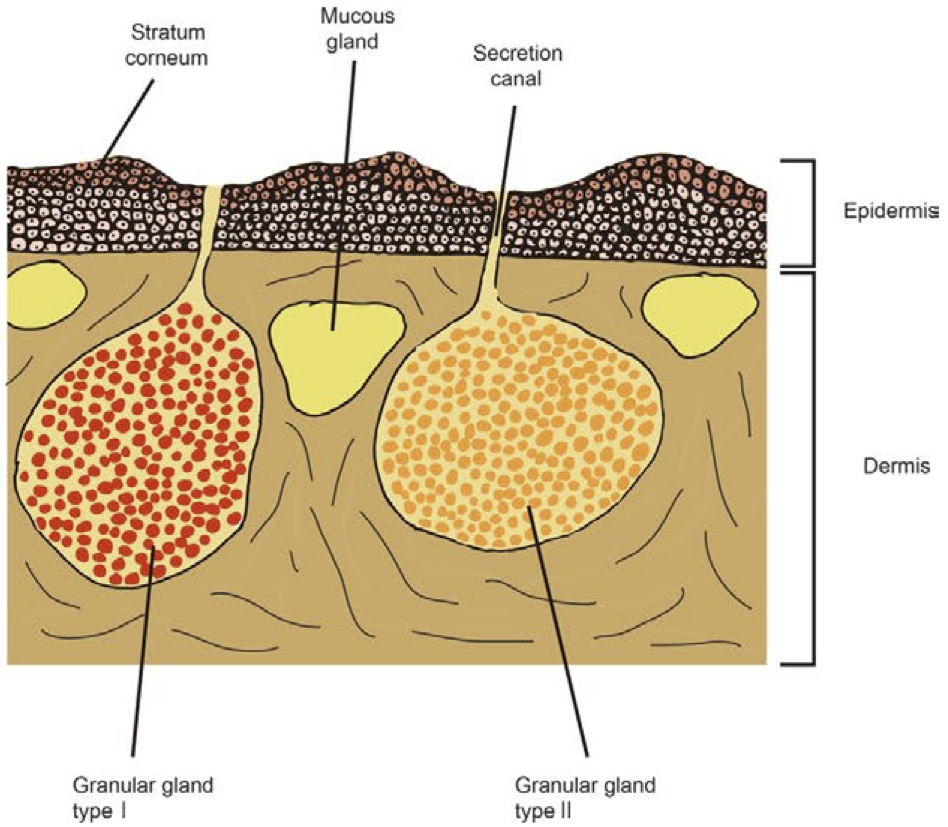
\includegraphics[width=0.48\textwidth]{figs/skin.png}
    \caption{Overall structure of the amphibian skin including a cornified layer (stratum corneum) in the epidermis and secretion glands (mucous glands and granular glands) in the dermis. Source: \citealt{yokoyama2018skin}, Fig. 1b.}
    \label{fig:skin}
\end{wrapfigure}

The defensive chemicals that occur in amphibians include alkaloids, biogenic amines, bufadienolides, peptides and proteins, steroids, and volatiles \citep{daly1987further, daly2005alkaloids, erspamer1994bioactive, daly2004biologically, pukala2006host}. These secretions are believed to function as an essential component of the innate immune system in defending against pathogens and parasites \citep{rivas2009amphibian, conlon2011contribution} and are also involved in complex antipredator mechanisms \citep{brodie1991predator}.

Given the importance of defensive compounds in diverse aspects of amphibian biology, studies of chemical defense are essential to understanding amphibian diversification. Researchers interested in amphibian chemical defense have oriented most of their studies toward natural products discovery. Nevertheless, such studies are severely limited not only in their ability to explain their findings (e.g., without understanding of amphibian phylogeny and ecology, variation in the kinds and amounts of defensive chemicals is unintelligible), but also the efficiency of their amphibian sampling \citep[e.g., phylogenetic trees provide roadmaps for natural products discovery; e.g.,~][]{smith2006venom}.

Starting during my Ph.D. studies, I have initiated an ongoing collaboration with research teams from different institutions (John Carroll University, University of Chicago, University of North Carolina, University of São Paulo, and Utah State University) which share the same overarching objective to understand the evolution of amphibian chemical defense by applying chemical, ecological, and phylogenetic concepts and methods. Within this context, my research effort has been towards reducing the gap between these research teams that are focused on basic research of non-model organisms and cutting-edge bioinformatic methods. With this proposal, I intend to focus on the evolution of an ancient hydrophilic alkaloid from the sea: a guanidine-based neurotoxin called tetrodotoxin (TTX).

\subsection{Chemistry, pharmacology, ecology, and biology of TTX}

Guanidine-based functional groups occur in many branches of chemistry, probably due to positive selection based on their ability to exist as neutral (guanidine), cationic (guanidinium), and anionic (guanidinate) entities \citep{tan2014chemistry}. Guanidines are neutral, nitrogen-containing compounds that synthetic organic chemistry uses widely as strong bases in synthetic organic chemistry \citep{berlinck2016chemistry}. Understanding the origins, biosynthesis, and biological activity of guanidine derivatives is a prolific area of research, primarily due to their antimicrobial properties \citep{zamperini2017identification}. Among guanidine natural products, two are conceivably originated from marine organisms and are known to be produced by blue-green algae: tetrodotoxin and saxitoxin. Tetrodotoxin is a secondary hydrophilic alkaloid metabolite bearing a guanidine group and unique pentacyclic structure (Fig.~\ref{fig:ttx}). 

\begin{wrapfigure}[18]{R}{0.5\textwidth}
    \centering
    \vspace{-\intextsep}\hspace*{-.75\columnsep}
    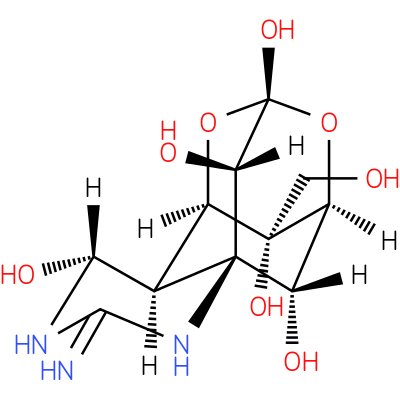
\includegraphics[width=0.48\textwidth]{figs/tetrodotoxin.png}
    \caption{Three-dimensional structure of the quinazoline alkaloid tetrodotoxin, C$_{11}$H$_{17}$N$_{3}$O$_{8}$. Source: ChEMBL.}
    \label{fig:ttx}
\end{wrapfigure}

2014 marked the 50$^{th}$ anniversary of the structure elucidation of TTX. Nonetheless, this is a small, highly functionalized, and intriguingly complex neurotoxin remains a subject of much research and will likely stay so for quite some time. The relevance of tetrodotoxin transcends the purely scientific realm as it also has significant implications for human health. For example, scientists continuously monitor tetrodotoxin and saxitoxin in seafood to avoid human intoxication \citep{berlinck2016chemistry}, and some expressed concern related to their potential (albeit unlikely) role in biotoxin warfare \citep[e.g.,][]{gorka2002biological, zhang2014effects, de2017neurological}. There is copious evidence to support the concern with how TTX can affect human health. On the one hand, ingestion of only about 2 mg of TTX (about 50–100 g of puffer fish) could be fatal by blocking the voltage-activated sodium channels, terminating nerve conduction and muscle action potentials and leading to progressive paralysis and respiratory failure \citep{de2017neurological}. On the other hand, this same neurotoxic activity has lead to the question of how TTX could serve as a therapeutic agent for pain \citep{nieto2012tetrodotoxin}. Tetrodotoxin is currently undergoing Phase III clinical trials for severe pain \citep{hagen2017tetrodotoxin}.

Numerous recent reviews summarize the extensive research into the chemistry, pharmacology, ecology, and biology of TTX \citep[e.g.,][]{narahashi2008tetrodotoxin, hanifin2010chemical, mandal2012tetrodotoxin, bane2014tetrodotoxin, berlinck2016chemistry}. Despite much investigation on TTX, its biosynthesis remains unknown. Moreover, scientists remain puzzled by the evolutionary mechanisms that allowed us to encounter this neurotoxin in different organisms that inhabit diverse ecosystems and possess no phylogenetic propinquity. So far, experts have isolated TTX from bacteria, dinoflagellates, and at least six phyla within Animalia including newts, pufferfish, marine mollusk, and terrestrial flatworms (for a list including organisms for which TTX presence is uncertain, see \citealt{chau2011origins}: Table 2). Some have argued that the diversity of species with TTX is evidence that symbiotic bacteria may be responsible for the production of this compound, which is further corroborated by experiments that cultured TTX-producing bacteria from the intestines of TTX-possessing marine vertebrates \citep[e.g.,][]{matsui2000purification}. However, several lines of evidence also suggest that bacteria are not the source of TTX \citep{hanifin2003tetrodotoxin, lehman2004no, salvitti2015first}. Therefore, one of the motivations of the current proposal is to shed light on the source of TTX in amphibians.

\subsection{Tetrodotoxin in amphibians}

First reported in amphibians of the genus \textit{Taricha} (order: Caudata, family: Salamandridae) (Fig.~\ref{fig:newt}) in the 1960s \citep[e.g.,~][]{mosher1964tarichatoxin}, the neurotoxin TTX is now known to occur in 27 species of amphibians and is suspected (on the basis of phylogeny and aposematic coloration and behavior) to occur in many more \citep{hanifin2010chemical}. Numerous recent reviews summarize the extensive research into the chemistry, pharmacology, ecology, and biology of TTX \citep[e.g.,~][]{narahashi2008tetrodotoxin, hanifin2010chemical, mandal2012tetrodotoxin, bane2014tetrodotoxin, berlinck2016chemistry} and the arms race between TTX-containing salamanders of the North American genus \textit{Taricha} and TTX-resistant garter snakes of the genus \textit{Thamnophis}  (Fig.~\ref{fig:race}) has become one of the classic models of coevolution \citep[for a historical account and summary see~][]{williams2010tetrodotoxin}.

\begin{figure}
  \begin{minipage}[b]{0.48\textwidth}
    \centering
    \vspace{-\intextsep}\hspace*{-.75\columnsep}
    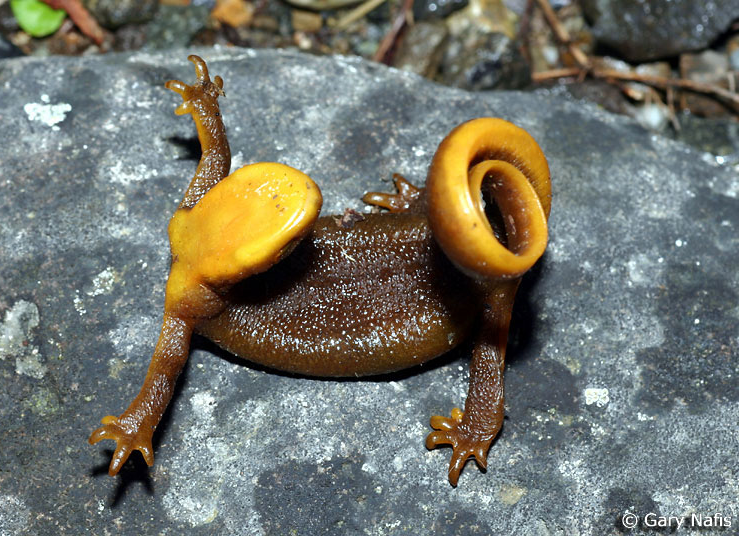
\includegraphics[width=\textwidth]{figs/taricha.png}
    \caption{Adult rough-skin newt \textit{Taricha granulosa} in defensive posture, showing the brightly-colored underside as a warning, and curling the tail. Credit: Gary Nafis.}
    \label{fig:newt}
  \end{minipage}
  \hfill
  \begin{minipage}[b]{0.48\textwidth}
    \centering
    \vspace{-\intextsep}\hspace*{-.75\columnsep}
    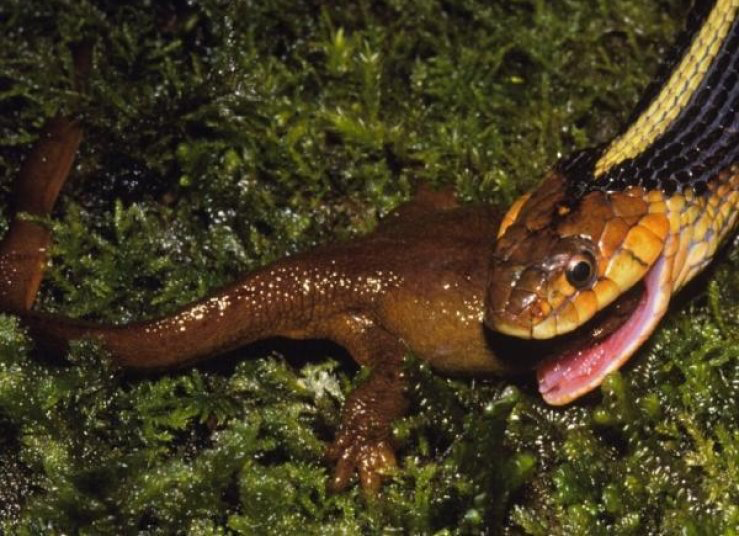
\includegraphics[width=\textwidth]{figs/thamnophis.png}
    \caption{Some garter snakes (\textit{Thamnophis sirtalis}) have evolved the ability to eat super-toxic newts (\textit{Taricha granulosa}). Credit: Edmund Brodie III.}
    \label{fig:race}
  \end{minipage}
\end{figure}

Little is known about TTX biosynthesis generally or its origin in amphibians specifically \citep{jal2015overview}. To tackle this, we initiated a collaboration with Dr. Edmund D. Brodie Jr. at Utah State University (USA) and designed the RNA sequencing experiment in an attempt to discover the genes responsible for the occurrence of TTX in \textit{Taricha granulosa}. The research plan, described in detail below, involves comparing the transcriptomes of populations of \textit{T. granulosa} with no TTX and with high levels of the toxin, to isolate genes potentially related to TTX biosynthesis and resistance. We will compare the list of candidate genes generated this way with public RNA data from pufferfish and original sequences of TTX-possessing frogs of the genus \textit{Brachycephalus} to increase resolution and corroborate our findings.